\documentclass[11pt,a4paper]{article}
\usepackage[margin=2cm]{geometry}
\usepackage{booktabs}
\usepackage{colortbl}
\usepackage{xcolor}
\usepackage{enumitem}
\usepackage{tikz}
\usepackage{tabularx}
\usepackage{multicol}
\usepackage{parskip}

% ── Colours ──
\definecolor{excellent}{HTML}{D1FAE5}
\definecolor{excellenttext}{HTML}{065F46}
\definecolor{good}{HTML}{DBEAFE}
\definecolor{goodtext}{HTML}{1E3A5F}
\definecolor{adequate}{HTML}{FEF9C3}
\definecolor{adequatetext}{HTML}{713F12}
\definecolor{below}{HTML}{FFEDD5}
\definecolor{belowtext}{HTML}{7C2D12}
\definecolor{poor}{HTML}{FECACA}
\definecolor{poortext}{HTML}{7F1D1D}

\definecolor{barintro}{HTML}{8B5CF6}
\definecolor{barconn}{HTML}{3B82F6}
\definecolor{barconc}{HTML}{06B6D4}
\definecolor{barrefs}{HTML}{F59E0B}
\definecolor{barwrit}{HTML}{F43F5E}

\definecolor{crediblebg}{HTML}{ECFDF5}
\definecolor{notcrediblebg}{HTML}{FEF2F2}
\definecolor{lightgray}{HTML}{F3F4F6}

\setlist[itemize]{nosep, left=0pt .. 1.5em}

% ── Tier row command: \tier{colour}{score}{description} ──
\newcommand{\tier}[3]{%
  \rowcolor{#1} \textbf{#2} & #3 \\
}

\pagestyle{empty}

\begin{document}

% ── Title ──
{\LARGE\bfseries Report Grading Rubric}\par\medskip

\bigskip

% ── Point Distribution Bar ──
{\small\textbf{Point Distribution}}\par\smallskip
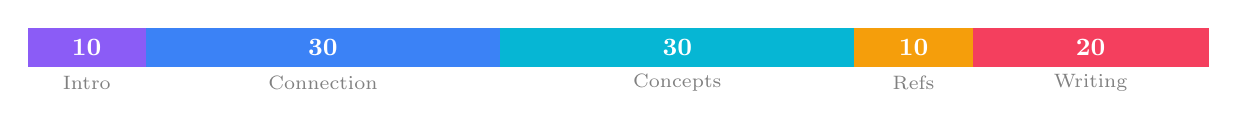
\begin{tikzpicture}
  \fill[barintro] (0,0) rectangle (1.5,0.5);
  \fill[barconn]  (1.5,0) rectangle (6,0.5);
  \fill[barconc]  (6,0) rectangle (10.5,0.5);
  \fill[barrefs]  (10.5,0) rectangle (12,0.5);
  \fill[barwrit]  (12,0) rectangle (15,0.5);
  \node[white,font=\small\bfseries] at (0.75,0.25) {10};
  \node[white,font=\small\bfseries] at (3.75,0.25) {30};
  \node[white,font=\small\bfseries] at (8.25,0.25) {30};
  \node[white,font=\small\bfseries] at (11.25,0.25) {10};
  \node[white,font=\small\bfseries] at (13.5,0.25) {20};
  \node[gray,font=\scriptsize] at (0.75,-0.2) {Intro};
  \node[gray,font=\scriptsize] at (3.75,-0.2) {Connection};
  \node[gray,font=\scriptsize] at (8.25,-0.2) {Concepts};
  \node[gray,font=\scriptsize] at (11.25,-0.2) {Refs};
  \node[gray,font=\scriptsize] at (13.5,-0.2) {Writing};
\end{tikzpicture}
\bigskip

% ── 1. Anime Introduction ──
\noindent\textbf{1.\ Anime Introduction} \hfill \colorbox{lightgray}{\small\textbf{10 pts}}\par\smallskip
\begin{tabularx}{\textwidth}{c X}
\toprule
\textbf{Score} & \textbf{Description} \\
\midrule
\tier{excellent}{10}{Names the work, summarizes plot in 3+ sentences, identifies cosmology-relevant themes}
\tier{good}{8}{Names the work, reasonable summary, but misses key themes}
\tier{adequate}{6}{Names the work with a brief 1--2 sentence summary}
\tier{below}{4}{Mentions the work but only superficial or inaccurate synopsis}
\tier{poor}{2}{Barely mentions the work; no meaningful summary}
\tier{poor}{0}{Missing or completely off-topic}
\bottomrule
\end{tabularx}
\bigskip

% ── 2. Cosmology-Anime Connection ──
\noindent\textbf{2.\ Cosmology-Anime Connection} \hfill \colorbox{lightgray}{\small\textbf{30 pts}}\par\smallskip
\begin{tabularx}{\textwidth}{c X}
\toprule
\textbf{Score} & \textbf{Description} \\
\midrule
\tier{excellent}{30}{3+ cosmological concepts identified with concrete scene references}
\tier{good}{25}{2 concepts with scene references, or 3+ concepts without specific scenes}
\tier{adequate}{20}{1--2 concepts with some scene context}
\tier{adequate}{15}{1 concept but the connection is vague or superficial}
\tier{below}{10}{Mentions cosmology in passing without tying it to the anime}
\tier{poor}{5}{Attempts a connection but it is incorrect or incoherent}
\tier{poor}{0}{No connection between the anime and cosmology}
\bottomrule
\end{tabularx}
\bigskip

% ── 3. Cosmological Concepts ──
\noindent\textbf{3.\ Cosmological Concepts} \hfill \colorbox{lightgray}{\small\textbf{30 pts}}\par\smallskip
\begin{tabularx}{\textwidth}{c X}
\toprule
\textbf{Score} & \textbf{Description} \\
\midrule
\tier{excellent}{30}{3+ real concepts explained accurately, goes beyond anime-level discussion}
\tier{good}{25}{2--3 concepts explained accurately with some depth}
\tier{adequate}{20}{1--2 concepts explained correctly at a basic level}
\tier{adequate}{15}{Attempts to explain concepts but contains minor inaccuracies}
\tier{below}{10}{Contains significant inaccuracies or misunderstandings}
\tier{poor}{5}{Mentions concepts by name only, with no real explanation}
\tier{poor}{0}{No cosmological content beyond the anime discussion}
\bottomrule
\end{tabularx}
\bigskip

\newpage

% ── 4. References ──
\noindent\textbf{4.\ References} \hfill \colorbox{lightgray}{\small\textbf{10 pts}}\par\smallskip
\begin{tabularx}{\textwidth}{c X}
\toprule
\textbf{Score} & \textbf{Description} \\
\midrule
\tier{excellent}{10}{3+ credible references, properly cited}
\tier{good}{8}{2 credible references with proper citations}
\tier{adequate}{6}{1 credible reference with proper citation}
\tier{below}{4}{References listed but none are credible or relevant}
\tier{poor}{2}{Only non-credible references (anime wikis, blogs, AI summaries)}
\tier{poor}{0}{No references}
\bottomrule
\end{tabularx}
\bigskip

% ── 5. Writing Quality ──
\noindent\textbf{5.\ Writing Quality} \hfill \colorbox{lightgray}{\small\textbf{20 pts}}\par\smallskip
\begin{tabularx}{\textwidth}{c X}
\toprule
\textbf{Score} & \textbf{Description} \\
\midrule
\tier{excellent}{20}{Clear structure (intro, body, conclusion), logical flow, minimal errors}
\tier{good}{16}{Mostly clear with minor structural issues or a few grammar errors}
\tier{adequate}{12}{Readable but disorganized or frequent grammar issues}
\tier{below}{8}{Poorly organized and difficult to follow}
\tier{poor}{4}{Mostly incoherent but some content is discernible}
\tier{poor}{0}{Incoherent or unreadable}
\bottomrule
\end{tabularx}
\bigskip

% ── Credible References ──
\noindent\textbf{What Counts as a Credible Reference?}\par
{\small\color{gray} Course lecture slides count as one reference regardless of how many slide decks are cited.}\par\smallskip
\begin{multicols}{2}
\colorbox{crediblebg}{\parbox{0.92\columnwidth}{%
\smallskip
{\small\bfseries\color{excellenttext} Credible}\par\smallskip
\begin{itemize}[leftmargin=1.2em]
  \item Peer-reviewed journal articles
  \item Textbooks (incl.\ Serjeant's \textit{Observational Cosmology})
  \item NASA / ESA / JAXA official pages
  \item ArXiv preprints
  \item Course lecture notes / slides
  \item PBS Space Time videos
\end{itemize}
\smallskip
}}

\columnbreak

\colorbox{notcrediblebg}{\parbox{0.92\columnwidth}{%
\smallskip
{\small\bfseries\color{poortext} Not Credible (on their own)}\par\smallskip
\begin{itemize}[leftmargin=1.2em]
  \item Wikipedia (OK only as supplementary)
  \item Anime wiki pages
  \item Personal blogs
  \item AI-generated summaries
\end{itemize}
\smallskip\smallskip\smallskip
}}
\end{multicols}
\bigskip

% ── Overall Grade Scale ──
\noindent\textbf{Overall Grade Scale}\par\smallskip
\begin{tabularx}{\textwidth}{*{5}{>{\centering\arraybackslash}X}}
\cellcolor{excellent}\textbf{\color{excellenttext}85--100} & \cellcolor{good}\textbf{\color{goodtext}70--84} & \cellcolor{adequate}\textbf{\color{adequatetext}55--69} & \cellcolor{below}\textbf{\color{belowtext}40--54} & \cellcolor{poor}\textbf{\color{poortext}0--39} \\
\cellcolor{excellent}{\small\color{excellenttext}Excellent} & \cellcolor{good}{\small\color{goodtext}Good} & \cellcolor{adequate}{\small\color{adequatetext}Adequate} & \cellcolor{below}{\small\color{belowtext}Below Exp.} & \cellcolor{poor}{\small\color{poortext}Insufficient} \\
\end{tabularx}

\vfill
\begin{center}
{\small\color{gray} Observational Cosmology \(\cdot\) NTHU}
\end{center}

\end{document}
